\documentclass[border=2mm]{standalone}
\usepackage{tikz}
\usetikzlibrary{decorations.fractals}
\begin{document}
\begin{tabular}{c}
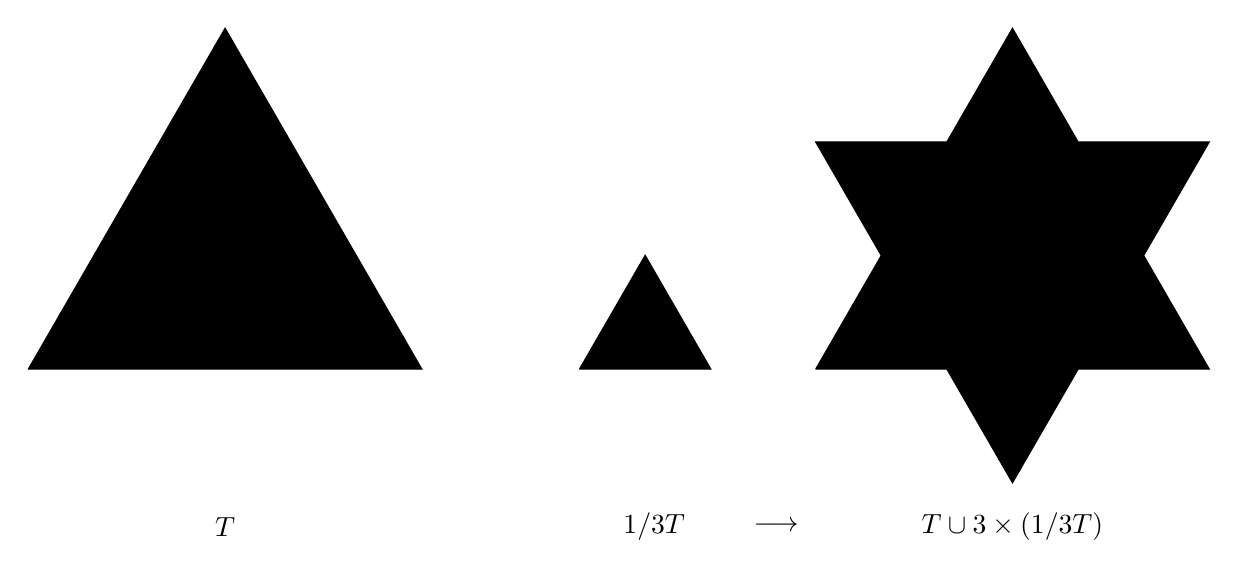
\begin{tikzpicture}[decoration=Koch snowflake]
   \draw[fill=black]  
        (0,0) -- ++(60:5)  -- ++(300:5) -- ++(180:5);
\node (C) at (2.5,-2) {$T$};
 \draw[fill=black]  
        (7,0) -- ++(60:1.67)  -- ++(300:1.67) -- ++(180:1.67);
\node (C) at (7.95,-2) {$1/3T$};
 \draw[fill=black] decorate {  
        (10,0) -- ++(60:5)  -- ++(300:5) -- ++(180:5)};
\node (C) at (12.5,-2) {$T\cup 3\times(1/3T)$};
\node (C) at (9.5,-2) {$\longrightarrow$};
\end{tikzpicture}\\
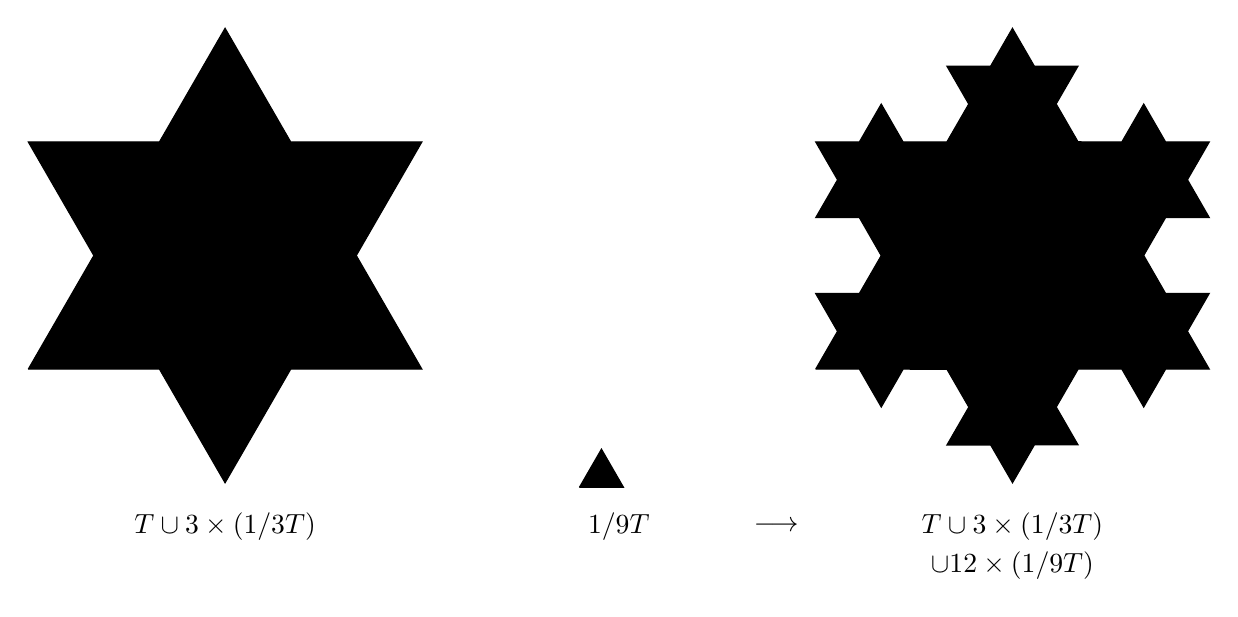
\begin{tikzpicture}[decoration=Koch snowflake]
   \draw[fill=black] decorate {  
        (0,0) -- ++(60:5)  -- ++(300:5) -- ++(180:5)};
\node (C) at (2.5,-2) {$T\cup 3\times(1/3T)$};
 \draw[fill=black]  
        (7,-1.5) -- ++(60:0.56)  -- ++(300:0.56) -- ++(180:0.56);
\node (C) at (7.5,-2) {$1/9T$};
 \draw[fill=black] decorate {  decorate{
        (10,0) -- ++(60:5)  -- ++(300:5) -- ++(180:5)}};
\node (C) at (12.5,-2) {$T\cup 3\times(1/3T)$};
\node (C) at (12.5,-2.5) {$\cup 12\times(1/9T)$};
\node (C) at (9.5,-2) {$\longrightarrow$};
 \end{tikzpicture}\\
 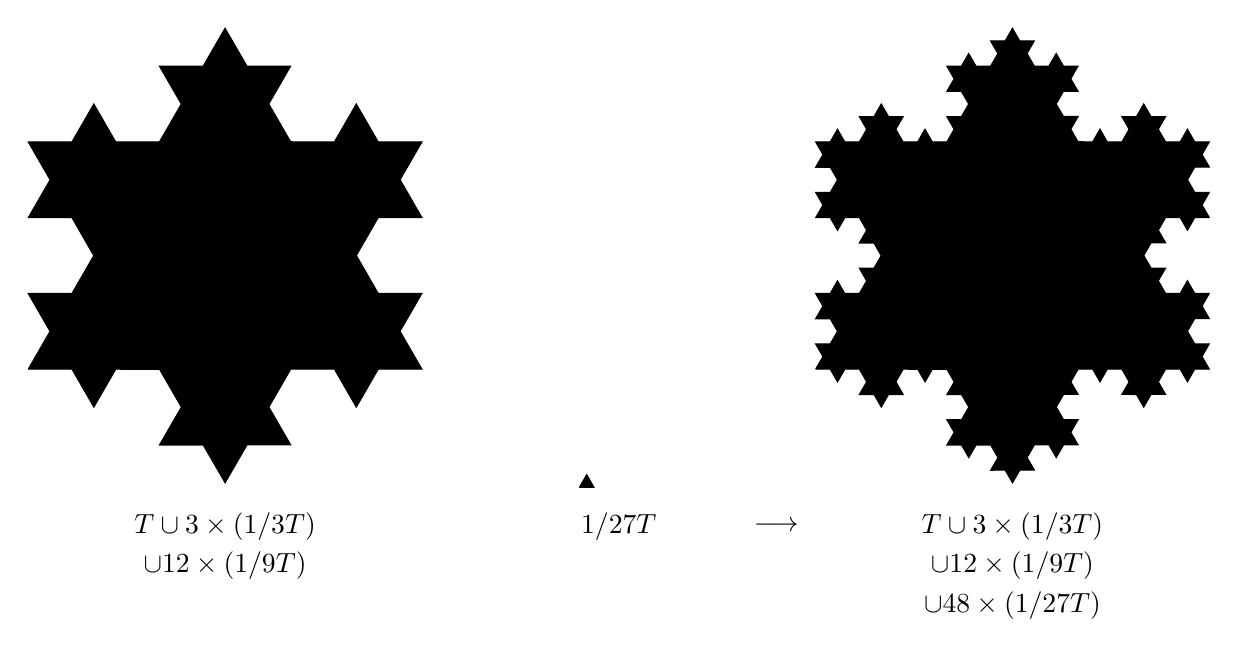
\begin{tikzpicture}[decoration=Koch snowflake]
   \draw[fill=black] decorate {  decorate { 
        (0,0) -- ++(60:5)  -- ++(300:5) -- ++(180:5)}};
\node (C) at (2.5,-2) {$T\cup 3\times(1/3T)$};
\node (C) at (2.5,-2.5) {$\cup 12\times(1/9T)$};
 \draw[fill=black]  
        (7,-1.5) -- ++(60:0.185)  -- ++(300:0.185) -- ++(180:0.185);
\node (C) at (7.5,-2) {$1/27T$};
 \draw[fill=black] decorate {  decorate{ decorate {
        (10,0) -- ++(60:5)  -- ++(300:5) -- ++(180:5)}}};
\node (C) at (12.5,-2) {$T\cup 3\times(1/3T)$};
\node (C) at (12.5,-2.5) {$\cup 12\times(1/9T)$};
\node (C) at (12.5,-3) {$\cup 48\times(1/27T)$};
\node (C) at (9.5,-2) {$\longrightarrow$};
 \end{tikzpicture}
\end{tabular} 
\end{document}